%% abtex2-modelo-trabalho-academico.tex, v-1.9.3 laurocesar
%% Copyright 2012-2015 by abnTeX2 group at http://abntex2.googlecode.com/ 
%% This work may be distributed and/or modified under the
%% conditions of the LaTeX Project Public License, either version 1.3
%% of this license or (at your option) any later version.
%% The latest version of this license is in
%%   http://www.latex-project.org/lppl.txt
%% and version 1.3 or later is part of all distributions of LaTeX
%% version 2005/12/01 or later.
%%
%% This work has the LPPL maintenance status `maintained'.
%% 
%% The Current Maintainer of this work is the abnTeX2 team, led
%% by Lauro César Araujo. Further information are available on 
%% http://abntex2.googlecode.com/
%%
%% This work consists of the files abntex2-modelo-trabalho-academico.tex,
%% abntex2-modelo-include-comandos and abntex2-modelo-references.bib
%%

% ------------------------------------------------------------------------
% ------------------------------------------------------------------------
% abnTeX2: Modelo de Trabalho Academico (tese de doutorado, dissertacao de
% mestrado e trabalhos monograficos em geral) em conformidade com 
% ABNT NBR 14724:2011: Informacao e documentacao - Trabalhos academicos -
% Apresentacao
% ------------------------------------------------------------------------
% ------------------------------------------------------------------------

\documentclass[
	% -- opções da classe memoir --
	12pt,				% tamanho da fonte
	openright,			% capítulos começam em pág ímpar (insere página vazia caso preciso)
	oneside,			% para impressão em verso e anverso. Oposto a oneside
	a4paper,			% tamanho do papel. 
	% -- opções da classe abntex2 --
	%chapter=TITLE,		% títulos de capítulos convertidos em letras maiúsculas
	%section=TITLE,		% títulos de seções convertidos em letras maiúsculas
	%subsection=TITLE,	% títulos de subseções convertidos em letras maiúsculas
	%subsubsection=TITLE,% títulos de subsubseções convertidos em letras maiúsculas
	% -- opções do pacote babel --
	english,			% idioma adicional para hifenização
	brazil				% o último idioma é o principal do documento
	]{abntex2}

% ---
% Pacotes básicos 
% ---
\usepackage{uarial}				% Usa a fonte Latin Modern			lmodern
\usepackage[T1]{fontenc}		% Selecao de codigos de fonte.
\usepackage[utf8]{inputenc}		% Codificacao do documento (conversão automática dos acentos)
\usepackage{lastpage}			% Usado pela Ficha catalográfica
\usepackage{indentfirst}		% Indenta o primeiro parágrafo de cada seção.
\usepackage{color}				% Controle das cores
\usepackage{graphicx}			% Inclusão de gráficos
\usepackage{microtype} 			% para melhorias de justificação
\usepackage{float}

% pacotes adicionados
\usepackage{amsmath}
\usepackage{amssymb,amsfonts,amsthm}
\usepackage{setspace}
% ---
		
% ---
% Pacotes adicionais, usados apenas no âmbito do Modelo Canônico do abnteX2
% ---
\usepackage{lipsum}				% para geração de dummy text
% ---
\usepackage{todonotes}
% ---
% Pacotes de citações
% ---
\usepackage[brazilian,hyperpageref]{backref}	 % Paginas com as citações na bibl
\usepackage[alf]{abntex2cite}	% Citações padrão ABNT


\renewcommand{\bf}[1]{\mathbf{#1}}
\renewcommand{\rm}[1]{\mathrm{#1}}


\usepackage{cite}
\renewcommand\citeleft{[}
\renewcommand\citeright{]}

% --- 
% CONFIGURAÇÕES DE PACOTES
% --- 
%\renewcommand{\imprimircapa}{
%\thispagestyle{empty}

\vfill
 \begin{center}
    
    {\large\bfseries INSTITUTO FEDERAL DE MATO GROSSO DO SUL} \\
    
    {\large\bfseries CAMPUS NAVIRAÍ}  \\ 

    \vspace*{1in}

    \vspace*{4cm}
    \noindent \\
    
    \large\bfseries{NOTAS DE AULA DE} \\
    \huge\bfseries{LINGUAGEM DE APRESENTAÇÃO E ESTRUTURAÇÃO DE CONTEÚDOS} \\ I
    
    \vspace*{4cm}
    
    \large{Prof. MSc. Luiz F. Picolo}
    
    \vfill
    \large\bfseries{NAVIRAÍ - MS} \\ 
    \vspace{0.2cm}
    \small Atualizado em \today
\end{center}

\normalsize


}


% \renewcommand{\imprimirfolhaderosto}{
% \include{folhaderosto}}


% ---
% Configurações do pacote backref
% Usado sem a opção hyperpageref de backref
\renewcommand{\backrefpagesname}{Citado na(s) página(s):~}
% Texto padrão antes do número das páginas
\renewcommand{\backref}{}
% Define os textos da citação
\renewcommand*{\backrefalt}[4]{
	\ifcase #1 %
		Nenhuma citação no texto.%
	\or
		Citado na página #2.%
	\else
		Citado #1 vezes nas páginas #2.%
	\fi}%
% ---
% \include{capa}

% ---
% Configurações de aparência do PDF final

% alterando o aspecto da cor azul
\definecolor{blue}{RGB}{41,5,195}

% informações do PDF
\makeatletter
\hypersetup{
     	%pagebackref=true,
		colorlinks=true,       		% false: boxed links; true: colored links
    	linkcolor=blue,          	% color of internal links
    	citecolor=black,        		% color of links to bibliography
    	filecolor=magenta,      		% color of file links
		urlcolor=blue,
		bookmarksdepth=4
}



\makeatother
% --- 

% --- 
% Espaçamentos entre linhas e parágrafos 
% --- 

% O tamanho do parágrafo é dado por:
\setlength{\parindent}{1.3cm}

% Controle do espaçamento entre um parágrafo e outro:
\setlength{\parskip}{0.2cm}  % tente também \onelineskip

% ---
% compila o indice
% ---
% \makeindex
% ---

% ----
% Início do documento
% ----
\begin{document}

% Seleciona o idioma do documento (conforme pacotes do babel)
%\selectlanguage{english}
\selectlanguage{brazil}

% Retira espaço extra obsoleto entre as frases.
\frenchspacing 

% ----------------------------------------------------------
% ELEMENTOS PRÉ-TEXTUAIS
% ----------------------------------------------------------
\pretextual

% ---
% Capa
% ---
\thispagestyle{empty}

\vfill
 \begin{center}
    
    {\large\bfseries INSTITUTO FEDERAL DE MATO GROSSO DO SUL} \\
    
    {\large\bfseries CAMPUS NAVIRAÍ}  \\ 

    \vspace*{1in}

    \vspace*{4cm}
    \noindent \\
    
    \large\bfseries{NOTAS DE AULA DE} \\
    \huge\bfseries{LINGUAGEM DE APRESENTAÇÃO E ESTRUTURAÇÃO DE CONTEÚDOS} \\ I
    
    \vspace*{4cm}
    
    \large{Prof. MSc. Luiz F. Picolo}
    
    \vfill
    \large\bfseries{NAVIRAÍ - MS} \\ 
    \vspace{0.2cm}
    \small Atualizado em \today
\end{center}

\normalsize



% ---

% ---
% Folha de rosto
% (o * indica que haverá a ficha bibliográfica)
% ---
% \imprimirfolhaderosto

% \include{ficha}
%\include{errata}
% \include{folhaaprova}
%\include{dedicatoria}
% \include{agradecimentos}
%\include{epigrafe}
% \include{resumos}
% ---
% inserir lista de ilustrações
% ---
% \pdfbookmark[0]{\listfigurename}{lof}
% \listoffigures*
% \cleardoublepage
%% ---

% ---
% inserir lista de tabelas
% ---
% \pdfbookmark[0]{\listtablename}{lot}
% \listoftables*
% \cleardoublepage
% ---
% \include{siglas}
% ---
% inserir o sumario
%% ---
% \pdfbookmark[0]{\contentsname}{toc}
% \tableofcontents*
% \cleardoublepage
%% ---



% ----------------------------------------------------------
% ELEMENTOS TEXTUAIS
% ----------------------------------------------------------
\textual

\chapter{Introdução}

\section{O que é JavaScript}

O JavaScript foi criado na década de 90 por \textbf{Brendan Eich} a serviço da 
Netscape (uma empresa de serviços de computadores nos EUA a qual era mais 
conhecida pelo seu navegador, o Netscape). Essa década foi um período de 
``revolução'', pois os navegadores ainda eram estáticos sendo o mais popular 
dessa época o Mosaic, da NCSA.

\begin{figure}[H]
  \centering
  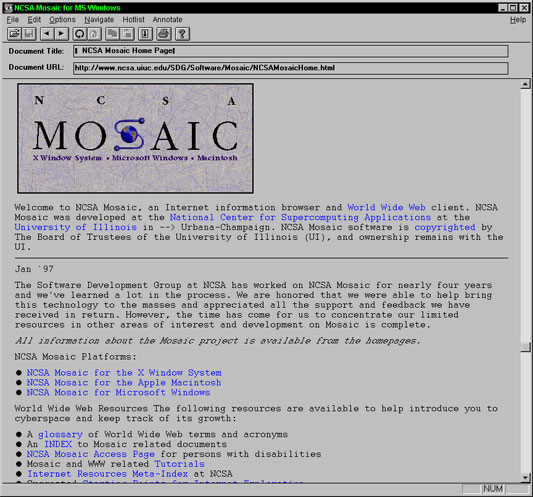
\includegraphics[scale=0.6]{imagens/mosaic_beta.jpg}
  \caption{NCSA Mosaic versão beta}
  \legend{Fonte: \cite{historyComputer}}
  \label{fig:historyComputer}
\end{figure}

O JavaScript foi introduzido em 1995 como uma forma de adicionar programas às 
páginas web do navegador Netscape. A linguagem, desde então, foi adotada por 
todos os outros grandes navegadores web que possuem interfaces gráficas. Ele 
tornou as aplicações modernas possíveis, fazendo com que você não tenha que 
recarregar a página inteira quando for necessário realizar interações diretas 
com a aplicação. Além disso, ele é usado em páginas web mais tradicionais, 
fornecendo diferentes maneiras de criar interatividade e inteligência \cite
{haverbeke2014eloquent}.

\section{ECMAScript ou JavaScript?}

Depois que o JavaScript foi adotado fora do Netscape, um documento padrão foi 
escrito para descrever a maneira na qual a linguagem deveria funcionar, 
garantindo que as diferentes partes dos softwares que afirmavam suportar 
JavaScript estavam, de fato, falando sobre a mesma linguagem. Esse documento é 
chamado de padrão ECMAScript, nomeado pela organização internacional Ecma, que 
foi responsável pela padronização. Na prática, os termos ECMAScript e 
JavaScript podem ser usados como sinônimos, pois são dois nomes para a mesma 
linguagem.

Na prática, existem diversos softwares que suportam JavaScript e possuem seu 
comportamente semelhante. Os navegadores, ou browsers, são exemplos destes 
tipos de software os quais implementam a linguagem por meio das especificações 
regidas pelo ECMAScript. Outro mais atual é o NodeJS ou simplesmente Node 
(https://nodejs.org/) que busca executar o JavaScript diretamente no servidor 
(Node será aprofundado em capítulos posteriores).

Para constatar este fato, execute o seguinte código no console em diferentes 
navegadores: 

\begin{lstlisting}
alert('Bem vindo(a) ao JavaScript')
\end{lstlisting}

O código acima possui o mesmo comportamento? Sim, o comportamento é o mesmo em 
todos os navegadores. Contudo, a forma gráfica com que é apresentado faz parte 
da implementação feita. Portanto, o desenvolvedor pode utilizar o JavaScript 
nos navegadores sem muito problema, pois eles seguem não ideias da equipe que o 
criou mas uma especificação que dita as regras de como determinadas funções 
devem se comportar.

\section{Versões do JavaScript ou edições ECMAScript}

Como foi visto, o ECMAScript é apenas a especificação. Contudo, ao estudar a 
linguagem é muito comum escutar a abreviação de ECMAScript, ou seja, ES. Assim, 
sempre que se ler ES seguido de um número, esse está fazendo referência a uma 
edição do ECMAScript. Atualmente, existem oito edições do ECMAScript publicadas,
sendo que, a partir de 2015, as edições começaram a receber o ano e não mais o 
número da edição.

\begin{enumerate}
  \item ECMAScript 1 (1997)	
  \item ECMAScript 2 (1998)	
  \item ECMAScript 3 (1999)	
  \item ECMAScript 4	Nunca foi lançada.
  \item ECMAScript 5 (2009)
    \begin{enumerate}[label*=\arabic*.]
    \item ECMAScript 5.1 (2011)
    \end{enumerate}
  \item ECMAScript 2015
  \item ECMAScript 2016
  \item ECMAScript 2017
  \item ECMAScript 2018
\end{enumerate}

\section{Conclusão}
Portanto, JavaScript se tornou a linguagem de programação mais popular no 
desenvolvimento Web sendo suportada por todos os navegadores e responsável por 
praticamente qualquer tipo de dinamismos em páginas web. Ao se usar todo o 
poder que ela tem para oferecer, pode-se chegar a resultados impressionantes. 
Alguns excelentes exemplos disso são aplicações Web complexas como Gmail, 
Google Maps e Google Docs. 

% \setcounter{chapter}{1}
\chapter{O que é User Experience (UX)}

\begin{flushright}
	\textit{
		UX é pesquisar sobre os usuários de modo que você possa dar para eles \\ o que eles precisam para conseguirem algo que querem.
	} \\
	
	\textbf{autor desconhecido}
\end{flushright}


No Capítulo \ref{cap:cap1}, nós realizamos a introdução sobre alguns conceitos norteadores da Interação Humano-Computador (IHC). No meio de todos os conceitos apresentados, algo se destaca em meio ao material apresentado, que é \textbf{usuário}. Sem dúvida, podemos afirmar que, o usuário, mediante sua interação com os sistemas computacionais, é a base para que uma área de estudo como IHC pudesse ser construída.

Já neste capítulo, iremos tratar não somente da interação do usuário por meios das interfaces, mas também da qualidade da sua experiência ao usar elas.

\section{Experiência do usuário}

Segundo \citeonline{teixeira2014introduccao}, a experiência do usuário existe desde que o mundo é mundo. Desde que as pessoas começaram a ``usar' objetos para realizar alguma tarefa podemos dizer que existe um contexto de experiências. Experiências são subjetivas. Cada pessoa tem uma experiência diferente ao usar um caixa eletrônico, um aplicativo, uma rede social, entre outros. Essa experiência, segundo \citeonline{teixeira2014introduccao} é influenciada por dois tipos de fatores: \textbf{humanos} e \textbf{externos} 

Como \textbf{fatores humanos} podemos citar as habilidade em usar caixas eletrônicos, por exemplo. Sua visão, sua habilidade motora, sua capacidade de ler e entender o que está escrito na tela, seu humor naquele momento, entre outros fatos. Já como \textbf{fatores externos}, podemos citar o horário do dia, o ambiente onde o caixa eletrônico está instalado, o fato de ter uma fila de pessoas atrás do utilizador, e assim por diante.

Assim, podemos dizer que o tema experiência do usuário é um tema bastante subjetivo. É difícil de maneira objetiva e direta dizer como desenhar uma experiência do usuário, mas é possível aprendermos como desenhar um produto, serviço ou ambiente que proporcione uma experiência satisfatória para alguém que os use, identificando todos os aspectos da interação do usuário com esse produto (ou serviço ou ambiente).

Portanto, a experiência do usuário está ligado a forma com que a pessoa se sente ao usar um produto. Ou mais formalmente, de acordo com a definição dada pela ISO 9241-210, são as respostas e percepções de uma pessoa resultantes do uso de um produto, sistema ou serviço.

UX designers trabalham para construir produtos que sejam fáceis de usar
(a tal \textbf{usabilidade}), reduzindo a fricção e permitindo que os usuários completem a tarefa desejada em menos tempo, com menos ruído e obstáculos.

\begin{figure}[H]
	\centering
	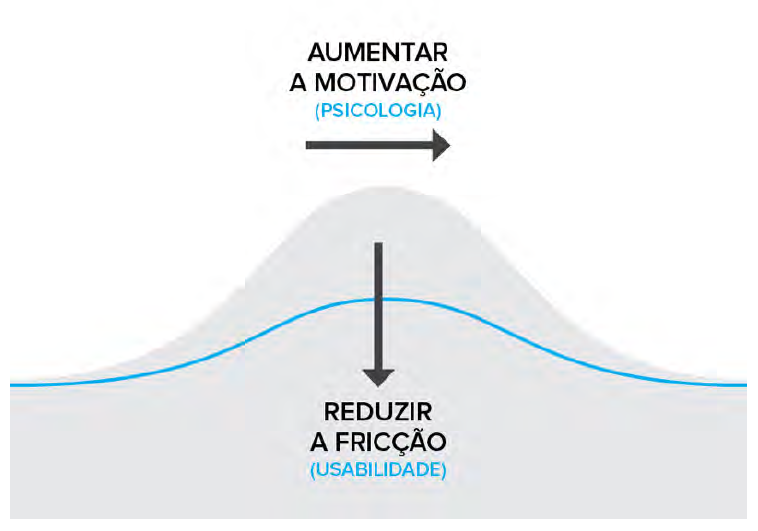
\includegraphics[scale=0.4]{imagens/aumento-friqcao.png}
	\caption{Stephen Anderson. Livro Seductive Interaction Design}
	%\legend{Fonte: \cite{IrlaRebelo}}
	%\label{fig:interface-interacao}
\end{figure}

\subsection{Usabilidade e a experiência do usuário}

Segundo a norma sobre requisitos de ergonomia, ISO 9241-11 (1998), define usabilidade como sendo: \textit{O grau em que um produto é usado por usuários específicos para atingir objetivos
específicos com \textbf{eficácia}, \textbf{eficiência} e \textbf{satisfação} em um contexto de uso
específico.}

\begin{itemize}
	\item \textbf{eficácia}: está relacionada com a capacidade de os usuários interagirem com o sistema para alcançar seus objetivos corretamente, conforme o esperado;
	
	\item \textbf{eficiência}:  está relacionada com os recursos necessários para os usuários
	interagirem com o sistema e alcançarem seus objetivos. Normalmente, os recursos
	necessários são tempo, mão de obra e materiais envolvidos; 
	
	\item \textbf{satisfação}: A norma também destaca
	a importância de considerarmos o grau de contentamento dos usuários com a experiência
	de usar o sistema interativo no contexto de uso para o qual foi projetado.
\end{itemize} 

De forma mais simplificada, segundo \cite{teixeira2014introduccao}: usablidade é garantir que as interfaces sejam fáceis de usar. Que o usuário consiga realizar uma tarefa sem transtorno ou demora em um número
razoável de passos, como também, toda informações sejam fáceis de entender e de fácil acesso. 

\section{Métodos e entregáveis em UX}

Quando falamos em métodos e entregáveis, os profissionais da área costumam ter uma série itens que gostam de utilizar: wireframes, sitemaps, user journeys, análise comparativa de funcionalidades, entre vários outros. Contudo, neste capítulo, vamos abordar apenas três os quais acreditamos ser os mais utilizados que são: \textbf{Brainstorming, Personas, Entrevistas com Stakeholders, Wireframes e Sitemaps}.

\subsection{Brainstorming}

O processo coletivo de geração de ideias, sem restrições. Uma sessão de \textit{brainstorming} busca
levantar de forma bastante livre um conjunto grande e abrangente de opiniões dos
participantes em torno de um tema. Os resultados dessa atividade podem alimentar
diretamente a especificação funcional e documentação de design \cite{barbosa2010IHC}.

\subsection{Personas}

Para \citeonline{teixeira2014introduccao}, personas é  um retrato do público-alvo que destaca dados demográficos, comportamentos,
necessidades e motivações por meio da criação de um personagem ficcional
baseado em \textit{insights} extraídos de pesquisa. Personas fazem com que os designers e desenvolvedores criem empatia com os consumidores durante o processo de design.

\begin{figure}[H]
	\centering
	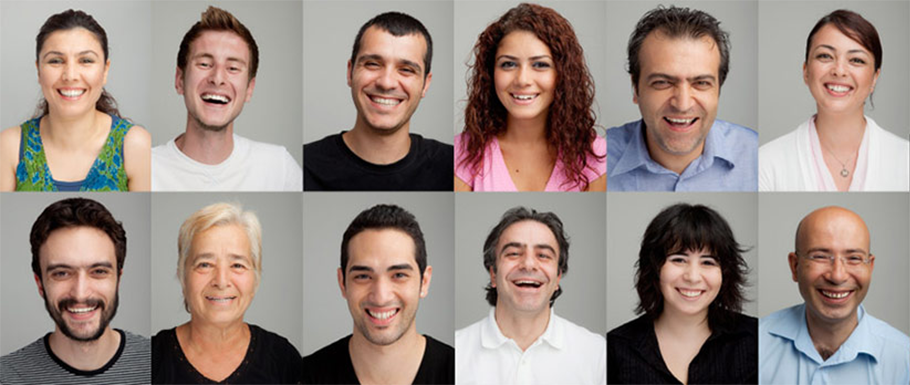
\includegraphics[scale=0.4]{imagens/personas-marketing.png}
	\caption{Exemplo de personas}
	\legend{Fonte: http://www.altgrupo.com.br/blog/marketing-digital-por-que-investir-no-uso-de-personas/}
	%\label{fig:interface-interacao}
\end{figure}

Para definir uma persona, \citeonline{courage2005understanding} enumera os seguintes elementos característicos:

\begin{itemize}
	\item \textbf{identidade}: dê a uma persona nome e sobrenome. Forneça uma idade e outros dados demográficos que seriam representativos do perfil do usuário. Inclua também uma foto, para tornar a persona ainda mais realista e memorável;
	\item \textbf{status}: defina se esta persona é primária, secundária, outro \textit{stakeholder} ou representa um antiusuário do seu sistema. Um antiusuário é alguém que não vai utilizar o produto e, portanto, não deve influenciar as decisões de projeto;
	\item \textbf{objetivos}: quais são os objetivos desta persona? Não se limite a objetivos relacionados ao seu produto específico;
	\item \textbf{habilidades}: qual é a especialidade da sua persona? Isso inclui educação, treinamento e competências específicas. Novamente, não se limite a detalhes relacionados ao seu produto específico;
	\item \textbf{tarefas}: em linhas gerais, quais as tarefas básicas ou críticas que a persona realiza? Qual é a frequência, importância e duração dessas tarefas?;
	\item \textbf{relacionamentos}: entender com quem a persona se relaciona é importante, pois ajuda a identificar outros \textit{stakeholders};
	\item \textbf{requisitos}: de que a persona precisa? Inclua citações que ajudam a dar mais vida a essas necessidades;
	\item \textbf{expectativas}: como a persona acredita que o produto funciona? Como ela organiza as informações no seu domínio ou trabalho?
\end{itemize}

Embora personas sejam fictícias, elas são definidas com rigor e detalhes para representar usuários ``típicos''. Elas são derivadas de um processo de investigação que levanta as características dos usuários e descreve seus perfis \cite{barbosa2010IHC}.

\subsubsection{Diferença entre persona e público-alvo}

Para \citeonline{riandutra2018} um erro bastante esta no fato da não diferenciação de personas de público-alvo. O público-alvo é algo mais genérico, abrangente, enquanto a persona é mais humanizada e personalizada.

Por exemplo, um público-alvo poderia ser: homens e mulheres, entre 30 e 40 anos, casados, com ensino médio completo, com renda mensal de até 15.000 reais. Têm até dois filhos e pretendem comprar uma casa de veraneio para a família.

Agora, um exemplo de persona: Patrícia, 31 anos, não tem filhos, é solteira, formada em design e pós-graduada em animação 3D. Busca ascensão profissional na empresa em que trabalha há cerca de dois anos. Gostaria de morar sozinha e procura formas de poupar dinheiro para as despesas de um novo apartamento.





% \chapter{Definição sobre JavaScript Object Notation (JSON)}\label{cap:cap3}

\begin{flushright}
	\textit{
		Um ladrão rouba um tesouro, mas não furta a inteligência. \\
		Uma crise destrói um herança, mas não uma profissão. \\ Não importa se você não tem dinheiro, você é uma pessoa rica, \\ pois possui o maior de todos os capitais: a sua inteligência. \\ Invista nela. \textbf{Estude}!.
	} \\
	
	\textbf{Augusto Cury}
\end{flushright}

JSON (JavaScript Object Notation) é um formato de intercâmbio de dados leve. É fácil para que seres humanos possam ler e escrever. É fácil para que as máquinas possam analisar e gerar. É baseado em um subconjunto do \textbf{Padrão de Linguagem de Programação JavaScript ECMA-262 3ª Edição} - Dezembro de 1999. JSON é um formato de texto completamente independente da linguagem, mas usa convenções que são familiares aos programadores da família C de linguagens, incluindo C, C ++, Java, JavaScript, Perl, Python e muitos outros. Essas propriedades tornam o JSON uma linguagem de intercâmbio de dados ideal\footnote{Para mais detalhes acesse: https://www.json.org/json-pt.html}.

Json também é um formato baseado em texto padrão para representar dados estruturados com base na sintaxe do objeto JavaScript. É comumente usado para transmitir dados em aplicativos da Web (por exemplo, enviar alguns dados do servidor para o cliente, para que possam ser exibidos em uma página da Web ou vice-versa). Você se deparará com isso com bastante frequência, portanto, neste artigo, oferecemos tudo o que você precisa para trabalhar com o JSON usando JavaScript, incluindo a análise do JSON para que você possa acessar os dados dentro dele e criar o JSON\footnote{Para mais detalhes acesse: \url{https://developer.mozilla.org/pt-BR/docs/Learn/JavaScript/Objects/JSON}}.

\section{Estrutura JSON}

Um JSON é uma string cujo formato se parece muito com o formato literal do objeto JavaScript. Você pode incluir os mesmos tipos de dados básicos dentro do JSON, como em um objeto JavaScript padrão — strings, números, matrizes, booleanos e outros literais de objeto. Isso permite que você construa uma hierarquia de dados. 

\begin{lstlisting}
let Retangulo = {
	"largura": 100,
	"altura": 100
}

let Retangulos = [
	{"largura": 100, "altura": 100},
	{"largura": 200, "altura": 200},
]
\end{lstlisting}

Assim, para realizar o acesso aos dados de um objeto Json, usamos a mesma notação \textbf{dot} / \textbf{bracket} usada em objetos literais.

\begin{lstlisting}
let Retangulo = {
	"largura": 100,
	"altura": 100
}

let Retangulos = [
	{"largura": 100, "altura": 100},
	{"largura": 200, "altura": 200},
]

console.log(Retangulo.largura)
console.log(Retangulo['largura'])

console.log(Retangulos[0].largura)
console.log(Retangulo[0]['largura'])
\end{lstlisting}

Contudo, o Json recebido venha em formato de String, ele deverá ser convertido para um objeto JavaScript. Assim, usando a função \textbf{JSON.parse()} podemos converter a string em um objeto, da seguinte forma:

\begin{lstlisting}
let retangulo = Json.parse('{"largura": 100, "altura": 100}')
console.log(Retangulo.largura)
\end{lstlisting}

\section{Exercícios de Fixação}

\begin{enumerate}
	\item No exercício 2.4 criamos uma classe \textbf{Noticia} que continha alguns atributos (titulo, dataDaPublicacao, resumo e texto) e uma outra classe \textbf{NoticiaDestaque} que continha, além dos atributos citados, um atributo imagem. Assim, baseando-se nos atributos listados, crie um arquivo \textbf{json} com nome \textbf{noticias.json} e atribua a ele uma lista de notícias no formato estudado. O arquivo deve conter no mínimo 5 notícias.
\end{enumerate}

\section{Obtendo JSON de um servidor web (Requisição Ajax)}

Para obter o JSON, vamos usar uma API chamada \textbf{XMLHttpRequest} (geralmente chamada de XHR). Esse é um objeto JavaScript muito útil que nos permite fazer solicitações de rede para recuperar recursos de um servidor via JavaScript (por exemplo, imagens, texto, JSON e até trechos de código HTML), o que significa que podemos atualizar pequenas seções de conteúdo sem ter que recarregar todo página. Isso levou a páginas da Web mais responsivas e parece empolgante, mas está além do escopo deste artigo ensinar isso com muito mais detalhes\footnote{Para mais detalhes acesse: \url{https://developer.mozilla.org/pt-BR/docs/Learn/JavaScript/Objects/JSON}}.

Para começar, vamos armazenar a URL do JSON que queremos recuperar em uma variável. Adicione o seguinte na parte inferior do seu código JavaScript:

\begin{lstlisting}
	let requestURL = 'https://raw.githubusercontent.com/luizpicolo/json-for-testing
/main/dragonball.json';
\end{lstlisting}

Para criar uma solicitação, precisamos criar uma nova instância de objeto de solicitação a partir do construtor XMLHttpRequest usando a palavra-chave new. Adicione o seguinte abaixo sua última linha:

\begin{lstlisting}
	let request = new XMLHttpRequest();
\end{lstlisting}

Agora precisamos abrir uma nova solicitação usando o método open() . Adicione a seguinte linha:

\begin{lstlisting}
	request.open('GET', requestURL);
\end{lstlisting}

Isso leva pelo menos dois parâmetros — existem outros parâmetros opcionais disponíveis. Nós só precisamos dos dois obrigatórios para este exemplo simples:

\begin{itemize}
	\item O método HTTP a ser usado ao fazer a solicitação de rede. Neste caso, GET é bom, pois estamos apenas recuperando alguns dados simples.
	\item O URL para fazer a solicitação — esta é a URL do arquivo JSON que armazenamos anteriormente.
\end{itemize}

Em seguida, adicione as duas linhas a seguir — aqui estamos definindo o  responseType como JSON, para que o XHR saiba que o servidor retornará o JSON e que isso deve ser convertido nos bastidores em um objeto JavaScript. Em seguida, enviamos a solicitação com o método send():

\begin{lstlisting}
	request.responseType = 'json';
	request.send();
\end{lstlisting}

A última parte desta seção envolve aguardar a resposta retornar do servidor e, em seguida, lidar com ela. Adicione o seguinte código abaixo do seu código anterior:

\begin{lstlisting}
	request.onload = function() {
		let personagens = request.response;
		
		const elemento = document.getElementById('list');
		let p1 = personagens.characters[0].name;
		elemento.insertAdjacentHTML('afterbegin', p1);
	}
\end{lstlisting}

\section{Exercícios de Fixação}

\begin{itemize}
	\item A partir do arquivo \textbf{noticias.json} criado no exercício anterior, e utilizando também as classes \textbf{Noticia} e \textbf{NoticiaDestaque} implementadas, leia e apresente no navegador as notícias contidas no arquivo \textbf{noticias.json}. Para tanto, você deve utilizar implementar a leitura do arquivo e, a partir dos dados, criar objetos e apresentar os mesmos no navegador. Abaixo segue o modelo base para o desenvolvimento do trabalho
\end{itemize}
% \chapter{Versionamento de Código}\label{cap:cap3}

\begin{flushright}
	\textit{
		Um ladrão rouba um tesouro, mas não furta a inteligência. \\
		Uma crise destrói um herança, mas não uma profissão. \\ Não importa se você não tem dinheiro, você é uma pessoa rica, \\ pois possui o maior de todos os capitais: a sua inteligência. \\ Invista nela. \textbf{Estude}!.
	} \\
	
	\textbf{Augusto Cury}
\end{flushright}

De forma simples, podemos dizer que o controle de versão é um sistema que registra as mudanças feitas em um arquivo ou um conjunto de arquivos ao longo do tempo de forma que você possa recuperar versões específicas para praticamente qualquer tipo de arquivo em um computador. 

Assim, esse capítulo, tem como objetivo proporcionar a você leitor(a) os pontos os quais julgamos mais importantes para compreender e praticar o controle de versão. Esse tipo de técnica é amplamente utilizado em ambientes de trabalho, nos quais, várias pessoas tem que trabalhar em um mesmo projeto. Assim, caso um erro aconteça, ou características nova surjam, os membros da equipe podem corrigir o problema de forma simples e rápida.  

\section{Projeto de banco de dados}


% \chapter{Autenticação e autorização com JWT}


% \input{cap6}

% ----------------------------------------------------------
% Finaliza a parte no bookmark do PDF
% para que se inicie o bookmark na raiz
% e adiciona espaço de parte no Sumário
% ----------------------------------------------------------
\phantompart

% ---
% Conclusão
% ---
%\chapter{Conclusão}
% ---

% ----------------------------------------------------------
% ELEMENTOS PÓS-TEXTUAIS
% ----------------------------------------------------------
\postextual
% ----------------------------------------------------------

% ----------------------------------------------------------
% Referências bibliográficas
% ----------------------------------------------------------
\bibliography{TCC.bib}

% ----------------------------------------------------------
% Glossário
% ----------------------------------------------------------
%
% Consulte o manual da classe abntex2 para orientações sobre o glossário.
%
%\glossary

%\include{apendices}

%\include{anexos}

%---------------------------------------------------------------------
% INDICE REMISSIVO
%---------------------------------------------------------------------
\phantompart
\printindex
%---------------------------------------------------------------------

\end{document}
